En esta sección, se detallan los diferentes experimentos que realizamos para medir el funcionamiento, la eficiencia y calidad de resultados, tanto de forma cuantitativa como cualitativa, de los métodos implementados.

Para lograr tal fin realizamos los siguientes tipos de experimentos:
\begin{itemize}
  \item Funcionamiento de los métodos implementados: Mostraremos que los métodos
        de interpolación funcionan correctamente comparandolos contra diferentes
        familias de funciones. A su vez, basandonos en las precisiones obtenidas,
        determinaremos el tamaño de bloque óptimo para el método Interpolación por Splines.
  \item Medición del ECM y PSNR de los métodos: Compararemos los errores obtenidos
        en varias instancias de pruebas para los distintos métodos.
  \item Medición de los tiempos de ejecución de los métodos: Compararemos los
        tiempos de ejecución utilizando los distintos métodos.
  \item Análisis cualitativos de los métodos, fenómeno de artifacts: Buscaremos
        reconocer defectos de interpolación en los videos generados.
\end{itemize}

Los videos utilizados para los diversos experimentos, fueron los siguientes:

\begin{itemize}
  \item \textbf{Video 1 - Skate}: 426x240, cantidad de cuadros originales: 151 , fps: 30, duracion: 5s.
  \item \textbf{Video 2 - Messi}: 426x240, cantidad de cuadros originales: 151, fps: 30, duracion: 5s.
  \item \textbf{Video 3 - Amanecer}: 426x240, cantidad de cuadros originales: 151, fps: 30, duracion: 5s.
\end{itemize}

Es importante mencionar que cada video representa una clase de video distinto, en donde el Video 1 contiene movimientos bruscos, el Video 2 cambios de camara, y el Video 3 movimientos suaves.

El motivo de estas elecciones se debe a la busqueda de diversos \textit{artifacts} a partir de las caracteristicas de cada clase.

\subsection{Detalles generales de la experimentación}

\begin{itemize}
    \item En los experimentos que se utilizaron números aleatorios, se generaron utilizando la función \textit{rand}, provista por la librería \texttt{stdlib.h}.
    \item La semilla para los números aleatorios se seteo utilizando el método \textit{srand(time(NULL))}, para evitar repeticiones de números en diferentes corridas.
    \item Las instancias de prueba fueron generadas con los archivos provistos por la cátedra. Adicionalmente, hicimos nuestras propias instancias emulando diferentes funciones (por ejemplo una función constante, lineal y cuadrática) para realizar el control de calidad de los métodos.
    \item Para medir los tiempos utilizamos la librería \textit{chrono} y medimos los resultados en nanosegundos.
    \item A su vez, utilizamos el nivel de optimización \textit{O2} de \textit{C++} a la hora de compilar el código.
    \item Todos los tests fueron corridos en la misma máquina bajo las mismas condiciones.
\end{itemize}


\subsection{Funcionamiento de los métodos implementados}\label{exp_funcionamiento}
En este experimento nuestro objetivo fue asegurarnos el correcto funcionamiento de nuestra implementación de la interpolación fragmentaria lineal, interpolación por splines, e interpolación por splines con tamaño de bloque fijo, tomando bloques de 2, 4, 8, 16, 32 y 64 cuadros.

Con este fin, realizamos una serie de tests que muestran el correcto funcionamiento de cada método para distintas familias de funciones:
\begin{itemize}
  \item Función constante.
  \item Función lineal.
  \item Función cuadrática.
  \item Función cúbica.
\end{itemize}

Luego, cada método de interpolación fue testeado contra cada una de las familias de funciones mencionadas de la siguiente forma:
\begin{itemize}
  \item Dada una familia de funciones, se generan aleatoriamente los coeficientes necesarios para definir una función de esa familia, i.e.: para una constante se genera solo el coeficiente independiente, mientras que para una cuadrática se generan 3 coeficientes.
    \item Una vez generada la función, se la evalua en un rango de valores para obtener un array de valores esperados.
    \item Luego, a partir del array de valores esperados se construye otro array quitandole elementos a intervalos fijos.
        Este nuevo array será el utilizado para realizar la interpolación, y lo que testearemos es la aproximación de  la
        interpolación a los elementos que quitamos.
    \item Una vez que tenemos la interpolación con cualquiera de los métodos mencionados, basta recorrer los elementos del array de valores esperados a la vez que evaluamos la interpolación obtenida.
        Para cada par de valores: esperado e interpolado, querremos ver que la diferencia absoluta es menor que un epsilon/cota de precision que
        definiremos dependiendo del método utilizado y la función a interpolar.
\end{itemize}

Es importante mencionar algunas carácterísticas de las instancias utilizadas:
\begin{itemize}
    \item Cantidad de puntos generados con la función(tamaño del array de valores esperados): 100
    \item Cantidad de puntos a interpolar: 50.
    \item Todos los coeficientes generados aleatoriamente están en el rango $[1,10]$,
        para evitar que las funciones generadas crezcan de forma desmedida.
\end{itemize}

Luego, se obtuvieron las siguientes cotas de precisión para los distintos métodos y funciones:

\begin{table}[H]
    \begin{tabular}{| c | c | c | c | c |}
    \hline
    {} & F. Constante & F. Lineal & F. Cuadrática & F. Cúbica \\ \hline
    Interpolación por Vecinos & 0.0001 & 10 & 1000 & 100000 \\
    Interpolación Fragmentaria Lineal & 0.0001 & 0.0001 & 10 & 1000 \\
    Interpolación por Splines (bloques tamaño 2) & 0.0001 & 0.0001 & 10 & 1000 \\
    Interpolación por Splines (bloques tamaño 4) & 0.0001 & 0.0001 & 5 & 500 \\
    Interpolación por Splines (bloques tamaño 8) & 0.0001 & 0.0001 & 1 & 200 \\
    Interpolación por Splines (bloques tamaño 16) & 0.0001 & 0.0001 & 1 & 200 \\
    Interpolación por Splines (bloques tamaño 32) & 0.0001 & 0.0001 & 1 & 200 \\
    Interpolación por Splines (bloques tamaño 64) & 0.0001 & 0.0001 & 1 & 200 \\
    Interpolación por Splines (1 solo bloque) & 0.0001 & 0.0001 & 1 & 200 \\
    \hline
    \end{tabular}
\end{table}

Analizando dichas cotas vemos que:
\begin{itemize}
    \item La Interpolación por Vecinos resulta razonable solo para funciones con muy
        poca variación (derivada a lo sumo constante). Esto se ve claramente en la
        cota de presición al interpolar una función Cuadrática.
    \item La Interpolación Fragmentaria Lineal es sustancialmente mejor que por Vecinos,
        y devuelve resultados razonables para funciones a lo sumo Cuadráticas.
    \item La Interpolación por Splines utilizando solo 2 puntos para cada bloque es
        equivalente a interpolar utilizando funciones lineales, y queda evidenciado al
        tener las mismas cotas de precisión.
    \item A partir de los tamaños de bloque 4 a 16, la Interpolación por Splines realiza
        una mejora ``asintótica'' de su cota de precisión.
    \item Entre los tamaños de bloque 16 a 64, no se notó una mejora significativa en la cota
        de precisión de la Interpolación por Splines.
    \item Al realizar Interpolación por Splines \textit{standard} (1 solo bloque),
        vemos que su cota de precisión concuerda con las cotas a las cuales ``convergen''
        los métodos de Interpolación por Splines con bloque de tamaño fijo. Es por esta razón
        que para los experimentos cualitativos, utilizaremos solamente la Interpolación
        por Splines \textit{standard}, y no la de tamaño de bloques fijo.
\end{itemize}

\subsection{Medición de los tiempos de ejecución de los métodos}
A partir de la implementaciones descriptas en la Sección \ref{Implementacion},
podemos inferir una complejidad temporal para cada método.

Sea $w$ la cantidad de filas de píxeles en cada imagen, $h$ la cantidad de
columnas, $i$ la cantidad de cuadros originales y sea $k$ la cantidad de
cuadros a agregar entre los originales:

Todos los metodos implementados tienen la misma complejidad temporal que es
 $\Theta(w*h*i*k*)$. Esta conclusion surge del hecho de que, en todos los casos,
 tenemos 4 ciclos anidados, en donde el primero se ejecuta $w$ veces, el segundo
 $h$ veces, el tercero $i$ veces, y el cuarto $k$ veces.
%\begin{itemize}
%  \item Vecino mas cercano: realizamos 4 ciclos anidados, en donde el primero se ejecuta $w$ veces, el segundo $h$ veces, el tercero $i$ veces, y el cuarto $k$ veces, la complejidad temporal del mismo es $\Theta(whik)$.
%  \item Interpolacion lineal: situacion identica a la de vecinos mas cercanos, por lo tanto su complejidad temporal es de $\Theta(whik)$.
%  \item Interpolacion por Splines: en este caso realizamos primero un ciclo que se ejecuta $w$ veces, dentro de este ciclamos $h$
%  \item Interpolacion por Splines con tamaño de bloque fijo:
%\end{itemize}
\newline
\newline
Para corroborar esta hipotesis planteamos un experimento con las siguientes caracteristicas:
\begin{itemize}
  \item Utilizamos el video provisto por la catedra llamado \textit{funnybaby}, el cual tiene 44 cuadros y es de 240x320.
  \item Solo medimos la resolucion del sistema, no su creacion o los respectivos pasajes de video a texto y viceversa.
  \item Dado que $w$, $h$ y $i$ son valores fijos que no podemos cambiar, variamos el $k$.
  \item Generamos instancias para valores de $k$ entre 1 y 6.
  \item Para cada valor distinto de $k$ generamos 4 instancias, cuyos valores vamos a promediar para mitigar los posibles valores distorsionados por algun procedimiento del procesador.
\end{itemize}

Los resultamos obtenidos fueron los siguientes:

\begin{center}
    \begin{tikzpicture}
    \begin{axis}[
        title={},
        xlabel={cantidad de cuadros agregados entre originales ($k$)},
        ylabel={tiempo (nanosegundos)},
        ylabel absolute,
        ylabel style={yshift=.3cm},
        scaled x ticks=false,
        scaled y ticks=false,
        enlargelimits=0.05,
        width=0.85\textwidth,
        height=0.45\textwidth,
        legend style={at={(1.015,1)},anchor=north west},
        no markers,
        thick,
        cycle list name=exotic
    ]
    \addplot[color=green] table[x index=0,y index=1]{datos/timelineal};
    \addplot[color=red] table[x index=0,y index=1]{datos/timevecinos};
    \addplot[color=blue] table[x index=0,y index=1]{datos/timesplines};
    \legend{Lineal, Vecinos, Splines}
    \end{axis}
    \end{tikzpicture}
\end{center}

Si tomamos los tiempos que arrojó la experimentación, y los dividimos por su respectivo $k$, obtenemos el siguiente resultado:

\begin{center}
    \begin{tikzpicture}
    \begin{axis}[
        title={},
        xlabel={cantidad de cuadros agregados entre originales ($k$)},
        ylabel={tiempo (nanosegundos) / $k$},
        ylabel absolute,
        ylabel style={yshift=.3cm},
        scaled x ticks=false,
        scaled y ticks=false,
        enlargelimits=0.05,
        width=0.85\textwidth,
        height=0.45\textwidth,
        legend style={at={(1.015,1)},anchor=north west},
        no markers,
        thick,
        cycle list name=exotic
    ]
    \addplot[color=green] table[x index=0,y index=2]{datos/timelineal};
    \addplot[color=red] table[x index=0,y index=2]{datos/timevecinos};
    \addplot[color=blue] table[x index=0,y index=2]{datos/timesplines};
    \legend{Lineal, Vecinos, Splines}
    \end{axis}
    \end{tikzpicture}
\end{center}

A partir de los graficos, queda de manifiesto que los metodos tienen la misma complejidad temporal, ya que solo difieren en una constante.

\subsection{Medición del ECM y PSNR de los métodos.}\label{ECM}
Sea $F$ un frame del vídeo real (ideal) , y $\bar{F}$ el mismo frame del vídeo efectivamente construidos por alguno de los métodos. Sea $m$ la cantidad de filas de píxeles en cada imagen y $n$ la cantidad de columnas.

Definimos el Error Cuadrático Medio, \texttt{ECM}, como el real dado por:
\begin{equation}
\texttt{ECM}(F,\bar{F}) = \frac{1}{mn}\sum_{i=1}^m\sum_{j = 1}^n |F_{k_{ij}} - \bar{F}_{k_{ij}}|^2
\end{equation}

A su vez definimos \emph{Peak to Signal Noise Ratio}, \texttt{PSNR}, como el real dado por:
\begin{equation}
\texttt{PSNR}(F,\bar{F}) = 10 \log_{10}\bigg(\frac{255^2}{\texttt{ECM}(F,\bar{F})}\bigg). \label{eq:psnr}
\end{equation}

Ambas medidas nos sirven para realizar un análisis cuantitativo de la calidad de los resultados obtenidos con los distintos métodos.

En este experimento utilizamos los videos propuestos al inicio de la experimentacion, variando la cantidad de cuadros que agregamos.
Dichos videos fueron elegidos especificamente para variar la dificultad de Interpolación:
\begin{itemize}
    \item El video \textbf{Amanecer} no contiene movimientos bruscos ni cambios de cámaras
        por lo que, para cualquier método, el error debería ser en lineas generales
        menor que pare el resto de los videos.
    \item El video \textbf{Skate} contiene movimientos bruscos pero no cambios de cámaras
        por lo que, se espera un mayor error que en el video anterior. Además,
        deberíamos ver un aumento del error en los frames donde hay movimientos
        bruscos.
    \item El video \textbf{Skate} contiene movimientos bruscos y cambios de cámaras
        por lo que, se espera un mayor error que en el resto de los videos. Además,
        deberíamos ver un aumento \textit{importante} del error en los frames
        donde se produce el cambio de cámara.
\end{itemize}

A continuación, presentaremos e iremos analizando los resultados obtenidos:

\subsubsection{ECM - Agregando 1 cuadro}

\begin{figure}[H]
	\centering
	\begin{tikzpicture}
		\begin{axis}[
			title={ },
			xlabel=Frame,
			ylabel=ECM,
			width=0.8\textwidth,
			height=0.5\textwidth,
			yticklabel style={/pgf/number format/fixed},
			scaled y ticks=false,
			legend style={at={(1.015,1)},anchor=north west},
			no markers,
			thick,
            cycle list name=exotic
		]
		\addplot table[x index=0,y index=1]{../src/exp/error-sunrise-vecinos1};
        \addplot[color=blue] table[x index=0,y index=1]{../src/exp/error-sunrise-lineal1};
        \addplot[color=red] table[x index=0,y index=1]{../src/exp/error-sunrise-spline1};
		\legend{Vecinos, Lineal, Spline}
		\end{axis}
	\end{tikzpicture}
	\caption{ECM para el video \textbf{Amanecer} al agregar 1 cuadro con distintos métodos de Interpolación.}
	\label{fig:ecm_sunrise_1}
\end{figure}

\begin{figure}[H]
	\centering
	\begin{tikzpicture}
		\begin{axis}[
			title={ },
			xlabel=Frame,
			ylabel=ECM,
			width=0.8\textwidth,
			height=0.5\textwidth,
			yticklabel style={/pgf/number format/fixed},
			scaled y ticks=false,
			legend style={at={(1.015,1)},anchor=north west},
			no markers,
			thick,
			cycle list name=exotic
		]
		\addplot table[x index=0,y index=1]{../src/exp/error-skate-vecinos1};
        \addplot[color=blue] table[x index=0,y index=1]{../src/exp/error-skate-lineal1};
        \addplot[color=red] table[x index=0,y index=1]{../src/exp/error-skate-spline1};
		\legend{Vecinos, Lineal, Spline}
		\end{axis}
	\end{tikzpicture}
	\caption{ECM para el video \textbf{Skate}  al agregar 1 cuadro con distintos métodos de Interpolación.}
	\label{fig:ecm_skate_1}
\end{figure}

\begin{figure}[H]
	\centering
	\begin{tikzpicture}
		\begin{axis}[
			title={ },
			xlabel=Frame,
			ylabel=ECM,
			width=0.8\textwidth,
			height=0.5\textwidth,
			yticklabel style={/pgf/number format/fixed},
			scaled y ticks=false,
			legend style={at={(1.015,1)},anchor=north west},
			no markers,
			thick,
			cycle list name=exotic
		]
		\addplot table[x index=0,y index=1]{../src/exp/error-messi-vecinos1};
        \addplot[color=blue] table[x index=0,y index=1]{../src/exp/error-messi-lineal1};
        \addplot[color=red] table[x index=0,y index=1]{../src/exp/error-messi-spline1};
		\legend{Vecinos, Lineal, Spline}
		\end{axis}
	\end{tikzpicture}
	\caption{ECM para el video \textbf{Messi}  al agregar 1 cuadro con distintos métodos de Interpolación.}
	\label{fig:ecm_messi_1}
\end{figure}

Viendo las Figuras \ref{fig:ecm_sunrise_1}, \ref{fig:ecm_skate_1} y \ref{fig:ecm_messi_1} podemos decir que:
\begin{itemize}
    \item La Interpolación por Vecinos obtiene consistentemente un mayor error que
        el resto de los métodos.
    \item La Interpolación Fragmentaria Lineal y la Interpolación por Splines obtienen
        en general un error similar, siendo la primera ligeramente mejor.
    \item El rango de error obtenido por todos los métodos en el video \textbf{Amanecer},
        es significativamente menor que en el resto de los videos. Además, se puede ver
        que el error obtenido en ese video es en cierta forma ``regular'', lo cual
        tiene sentido ya que tiene movimientos suaves y repetitivos.
    \item El rango de error obtenido por todos los métodos en los videos \textbf{Skate} y \textbf{Messi},
        son similares, y ambos mayores al rango obtenido en el video \textbf{Amanecer}.
    \item El error obtenido en el video \textbf{Skate} es bastante irregular
        al compararlo con el video \textbf{Amanecer}, encontrandose un pico de error
        en el movimiento más brusco del video.
    \item A diferencia del caso anterior, el error obtenido en el video \textbf{Messi}
        es bastante regular, a excepción del pico de error que encontramos cuando
        ocurre el cambio de cámara, el cual es notorio para todos los métodos.
\end{itemize}

\subsubsection{PSNR - Agregando 1 cuadro}
\begin{figure}[H]
	\centering
	\begin{tikzpicture}
		\begin{axis}[
			title={ },
			xlabel=Frame,
			ylabel=PSNR,
			width=0.8\textwidth,
			height=0.5\textwidth,
			yticklabel style={/pgf/number format/fixed},
			scaled y ticks=false,
			legend style={at={(1.015,1)},anchor=north west},
			no markers,
			thick,
			cycle list name=exotic
		]
		\addplot table[x index=0,y index=2]{../src/exp/error-sunrise-vecinos1};
        \addplot[color=blue] table[x index=0,y index=2]{../src/exp/error-sunrise-lineal1};
        \addplot[color=red] table[x index=0,y index=2]{../src/exp/error-sunrise-spline1};
		\legend{Vecinos, Lineal, Spline}
		\end{axis}
	\end{tikzpicture}
	\caption{PSNR para el video \textbf{Amanecer} al agregar 1 cuadro con distintos métodos de Interpolación.}
	\label{fig:psnr_sunrise_1}
\end{figure}

\begin{figure}[H]
	\centering
	\begin{tikzpicture}
		\begin{axis}[
			title={ },
			xlabel=Frame,
			ylabel=PSNR,
			width=0.8\textwidth,
			height=0.5\textwidth,
			yticklabel style={/pgf/number format/fixed},
			scaled y ticks=false,
			legend style={at={(1.015,1)},anchor=north west},
			no markers,
			thick,
			cycle list name=exotic
		]
		\addplot table[x index=0,y index=2]{../src/exp/error-skate-vecinos1};
        \addplot[color=blue] table[x index=0,y index=2]{../src/exp/error-skate-lineal1};
        \addplot[color=red] table[x index=0,y index=2]{../src/exp/error-skate-spline1};
		\legend{Vecinos, Lineal, Spline}
		\end{axis}
	\end{tikzpicture}
	\caption{PSNR para el video \textbf{Skate} al agregar 1 cuadro con distintos métodos de Interpolación.}
	\label{fig:psnr_skate_1}
\end{figure}

\begin{figure}[H]
	\centering
	\begin{tikzpicture}
		\begin{axis}[
			title={ },
			xlabel=Frame,
			ylabel=PSNR,
			width=0.8\textwidth,
			height=0.5\textwidth,
			yticklabel style={/pgf/number format/fixed},
			scaled y ticks=false,
			legend style={at={(1.015,1)},anchor=north west},
			no markers,
			thick,
			cycle list name=exotic
		]
		\addplot table[x index=0,y index=2]{../src/exp/error-messi-vecinos1};
        \addplot[color=blue] table[x index=0,y index=2]{../src/exp/error-messi-lineal1};
        \addplot[color=red] table[x index=0,y index=2]{../src/exp/error-messi-spline1};
		\legend{Vecinos, Lineal, Spline}
		\end{axis}
	\end{tikzpicture}
	\caption{PSNR para el video \textbf{Messi} al agregar 1 cuadro con distintos métodos de Interpolación.}
	\label{fig:psnr_messi_1}
\end{figure}

Sabiendo que, mientras más grande es el \texttt{ECM} más chico es el \texttt{PSNR},
encontramos que la información provista por este último no aporta nuevos elementos
al análisis, ya que se condice con lo análizado previamente utilizando el \texttt{ECM}.

\subsubsection{ECM - Agregando 5 cuadros}

\begin{figure}[H]
	\centering
	\begin{tikzpicture}
		\begin{axis}[
			title={ },
			xlabel=Frame,
			ylabel=ECM,
			width=0.8\textwidth,
			height=0.5\textwidth,
			yticklabel style={/pgf/number format/fixed},
			scaled y ticks=false,
			legend style={at={(1.015,1)},anchor=north west},
			no markers,
			thick,
			cycle list name=exotic
		]
		\addplot table[x index=0,y index=1]{../src/exp/error-sunrise-vecinos5};
        \addplot[color=blue] table[x index=0,y index=1]{../src/exp/error-sunrise-lineal5};
        \addplot[color=red] table[x index=0,y index=1]{../src/exp/error-sunrise-spline5};
		\legend{Vecinos, Lineal, Spline}
		\end{axis}
	\end{tikzpicture}
	\caption{ECM para el video \textbf{Amanecer} al agregar 5 cuadros con distintos métodos de Interpolación.}
	\label{fig:ecm_sunrise_5}
\end{figure}

\begin{figure}[H]
	\centering
	\begin{tikzpicture}
		\begin{axis}[
			title={ },
			xlabel=Frame,
			ylabel=ECM,
			width=0.8\textwidth,
			height=0.5\textwidth,
			yticklabel style={/pgf/number format/fixed},
			scaled y ticks=false,
			legend style={at={(1.015,1)},anchor=north west},
			no markers,
			thick,
			cycle list name=exotic
		]
		\addplot table[x index=0,y index=1]{../src/exp/error-skate-vecinos5};
        \addplot[color=blue] table[x index=0,y index=1]{../src/exp/error-skate-lineal5};
        \addplot[color=red] table[x index=0,y index=1]{../src/exp/error-skate-spline5};
		\legend{Vecinos, Lineal, Spline}
		\end{axis}
	\end{tikzpicture}
	\caption{ECM para el video \textbf{Skate} al agregar 5 cuadros con distintos métodos de Interpolación.}
	\label{fig:ecm_skate_5}
\end{figure}

\begin{figure}[H]
	\centering
	\begin{tikzpicture}
		\begin{axis}[
			title={ },
			xlabel=Frame,
			ylabel=ECM,
			width=0.8\textwidth,
			height=0.5\textwidth,
			yticklabel style={/pgf/number format/fixed},
			scaled y ticks=false,
			legend style={at={(1.015,1)},anchor=north west},
			no markers,
			thick,
			cycle list name=exotic
		]
		\addplot table[x index=0,y index=1]{../src/exp/error-messi-vecinos5};
        \addplot[color=blue] table[x index=0,y index=1]{../src/exp/error-messi-lineal5};
        \addplot[color=red] table[x index=0,y index=1]{../src/exp/error-messi-spline5};
		\legend{Vecinos, Lineal, Spline}
		\end{axis}
	\end{tikzpicture}
	\caption{ECM para el video \textbf{Messi} al agregar 5 cuadros con distintos métodos de Interpolación.}
	\label{fig:ecm_messi_5}
\end{figure}

Viendo las Figuras \ref{fig:ecm_sunrise_5}, \ref{fig:ecm_skate_5} y \ref{fig:ecm_messi_5} podemos decir que:
\begin{itemize}
    \item El comportamiento general de los métodos para cada video no varió con respecto
        al escenario en el cual agregabamos 1 cuadro. Los análisis de movimiento brusco y
        cambios de cámaras se reafirman.
    \item En lineas generales, y en todos los videos, el error se incrementó con respecto al
        escenario en el cual agregabamos 1 cuadro, a excepción del método de Interpolación
        por Vecinos, que mantiene su rango de error.
\end{itemize}

\subsubsection{PSNR - Agregando 5 cuadros}
\begin{figure}[H]
	\centering
	\begin{tikzpicture}
		\begin{axis}[
			title={ },
			xlabel=Frame,
			ylabel=PSNR,
			width=0.8\textwidth,
			height=0.5\textwidth,
			yticklabel style={/pgf/number format/fixed},
			scaled y ticks=false,
			legend style={at={(1.015,1)},anchor=north west},
			no markers,
			thick,
			cycle list name=exotic
		]
		\addplot table[x index=0,y index=2]{../src/exp/error-sunrise-vecinos5};
        \addplot[color=blue] table[x index=0,y index=2]{../src/exp/error-sunrise-lineal5};
        \addplot[color=red] table[x index=0,y index=2]{../src/exp/error-sunrise-spline5};
		\legend{Vecinos, Lineal, Spline}
		\end{axis}
	\end{tikzpicture}
	\caption{PSNR para el video \textbf{Amanecer} al agregar 5 cuadros con distintos métodos de Interpolación.}
	\label{fig:psnr_sunrise_5}
\end{figure}

\begin{figure}[H]
	\centering
	\begin{tikzpicture}
		\begin{axis}[
			title={ },
			xlabel=Frame,
			ylabel=PSNR,
			width=0.8\textwidth,
			height=0.5\textwidth,
			yticklabel style={/pgf/number format/fixed},
			scaled y ticks=false,
			legend style={at={(1.015,1)},anchor=north west},
			no markers,
			thick,
			cycle list name=exotic
		]
		\addplot table[x index=0,y index=2]{../src/exp/error-skate-vecinos5};
        \addplot[color=blue] table[x index=0,y index=2]{../src/exp/error-skate-lineal5};
        \addplot[color=red] table[x index=0,y index=2]{../src/exp/error-skate-spline5};
		\legend{Vecinos, Lineal, Spline}
		\end{axis}
	\end{tikzpicture}
	\caption{PSNR para el video \textbf{Skate} al agregar 5 cuadros con distintos métodos de Interpolación.}
	\label{fig:psnr_skate_5}
\end{figure}

\begin{figure}[H]
	\centering
	\begin{tikzpicture}
		\begin{axis}[
			title={ },
			xlabel=Frame,
			ylabel=PSNR,
			width=0.8\textwidth,
			height=0.5\textwidth,
			yticklabel style={/pgf/number format/fixed},
			scaled y ticks=false,
			legend style={at={(1.015,1)},anchor=north west},
			no markers,
			thick,
			cycle list name=exotic
		]
		\addplot table[x index=0,y index=2]{../src/exp/error-messi-vecinos5};
        \addplot[color=blue] table[x index=0,y index=2]{../src/exp/error-messi-lineal5};
        \addplot[color=red] table[x index=0,y index=2]{../src/exp/error-messi-spline5};
		\legend{Vecinos, Lineal, Spline}
		\end{axis}
	\end{tikzpicture}
	\caption{PSNR para el video \textbf{Messi} al agregar 5 cuadros con distintos métodos de Interpolación.}
	\label{fig:psnr_messi_5}
\end{figure}

Sabiendo que, mientras más grande es el \texttt{ECM} más chico es el \texttt{PSNR},
encontramos que la información provista por este último no aporta nuevos elementos
al análisis, ya que se condice con lo análizado previamente utilizando el \texttt{ECM}.

\subsubsection{Conclusiones}

En base a lo análizado, podemos concluir que:

\begin{itemize}
    \item El error máximo cometido por el método de Interpolación por Vecinos, en comparación
        con los otros dos, lo hace inusable en la mayoría de los casos, y empeora a medida
        que agregamos más cuadros.
    \item Si bien en el Experimento de la Sección \ref{exp_funcionamiento} pudimos lograr una
        mayor precisión con la Interpolación por Splines que con la Interpolación Fragmentaria Lineal,
        no sucedió lo mismo cuando aplicamos los métodos a la interpolación de videos.
        En este escenario, los métodos obtuvieron errores muy similares, siendo la Interpolación
        Fragmentaria Lineal mejor en algunos casos.

        Esto lo atribuimos a que los píxeles de de los videos no respetan ninguna familia de funciones,
        obviamente, y por lo tanto la función que infiere la Interpolación por Splines
        no es sustancialmente mejor que la obtenida mediante Interpolación Fragmentaria Lineal.

        Sin embargo, ya que las cotas de precisión definidas previamente no nos permitieron
        proyectar que la Interpolación por Splines iba a dar resultados similares a la
        Interpolación Fragmentaria Lineal, queda la duda de si la Interpolación por Splines
        de tamaño de bloque fijo puede dar mejores resultados. Para eso, haremos un
        experimento extra a continuación para comparar el error de dichos métodos.
    \item El video con movimientos suaves es mucho más sencillo de interpolar que los demás, y
        permite que incluso el método de Interpolación por Vecinos logre errores bajos.
        Al ir agregando movimientos bruscos y cambios de camaras, los videos se vuelven más
        difíciles de interpolar, aumentando el error obtenido con los distintos métodos.
\end{itemize}

\subsubsection{Interpolación por Splines: bloques de tamaño variable vs fijo}

A continuación presentamos los resultados de comparar los errores de los siguientes métodos, solo para el video \textbf{Messi}:
\begin{itemize}
    \item Interpolación por Splines \textit{standard}, o de bloque variable.
    \item Interpolación por Splines (bloques de tamaño 2)
    \item Interpolación por Splines (bloques de tamaño 8)
    \item Interpolación por Splines (bloques de tamaño 32)
\end{itemize}

\begin{figure}[H]
	\centering
	\begin{tikzpicture}
		\begin{axis}[
			title={ },
			xlabel=Frame,
			ylabel=ECM,
			width=0.8\textwidth,
			height=0.5\textwidth,
			yticklabel style={/pgf/number format/fixed},
			scaled y ticks=false,
			legend style={at={(1.015,1)},anchor=north west},
			no markers,
			thick,
			cycle list name=exotic
		]
		\addplot table[x index=0,y index=1]{../src/exp/error-messi-multisplines1-b2};
        %\addplot table[x index=0,y index=1]{../src/exp/error-messi-multisplines1-b4};
        \addplot table[x index=0,y index=1]{../src/exp/error-messi-multisplines1-b8};
        %\addplot table[x index=0,y index=1]{../src/exp/error-messi-multisplines1-b16};
        \addplot table[x index=0,y index=1]{../src/exp/error-messi-multisplines1-b32};
        %\addplot table[x index=0,y index=1]{../src/exp/error-messi-multisplines1-b64};
        \addplot table[x index=0,y index=1]{../src/exp/error-messi-spline1};
		%\legend{B2, B4, B8, B16, B32, B64, Standard}
        \legend{B2, B8, B32, Standard}
		\end{axis}
	\end{tikzpicture}
	\caption{ECM para el video \textbf{Messi}  al agregar 1 cuadro con variantes del método de Interpolación por Splines.}
	\label{fig:ecm_splines_messi_1}
\end{figure}

\begin{figure}[H]
	\centering
	\begin{tikzpicture}
		\begin{axis}[
			title={ },
			xlabel=Frame,
			ylabel=ECM,
			width=0.8\textwidth,
			height=0.5\textwidth,
			yticklabel style={/pgf/number format/fixed},
			scaled y ticks=false,
			legend style={at={(1.015,1)},anchor=north west},
			no markers,
			thick,
			cycle list name=exotic
		]
		%\addplot table[x index=0,y index=1]{../src/exp/error-messi-multisplines1-b2};
        %\addplot table[x index=0,y index=1]{../src/exp/error-messi-multisplines1-b4};
        %\addplot table[x index=0,y index=1]{../src/exp/error-messi-multisplines1-b8};
        %\addplot table[x index=0,y index=1]{../src/exp/error-messi-multisplines1-b16};
        \addplot table[x index=0,y index=1]{../src/exp/error-messi-multisplines1-b32};
        %\addplot table[x index=0,y index=1]{../src/exp/error-messi-multisplines1-b64};
        \addplot table[x index=0,y index=1]{../src/exp/error-messi-spline1};
		%\legend{B2, B4, B8, B16, B32, B64, Standard}
        \legend{B32, Standard}
		\end{axis}
	\end{tikzpicture}
	\caption{ECM para el video \textbf{Messi}  al agregar 1 cuadro con variantes del método de Interpolación por Splines.}
	\label{fig:ecm_splines_messi_1_bis}
\end{figure}

\begin{figure}[H]
	\centering
	\begin{tikzpicture}
		\begin{axis}[
			title={ },
			xlabel=Frame,
			ylabel=ECM,
			width=0.8\textwidth,
			height=0.5\textwidth,
			yticklabel style={/pgf/number format/fixed},
			scaled y ticks=false,
			legend style={at={(1.015,1)},anchor=north west},
			no markers,
			thick,
			cycle list name=exotic
		]
        \addplot table[x index=0,y index=1]{../src/exp/error-messi-multisplines5-b2};
        %\addplot table[x index=0,y index=1]{../src/exp/error-messi-multisplines5-b4};
        \addplot table[x index=0,y index=1]{../src/exp/error-messi-multisplines5-b8};
        %\addplot table[x index=0,y index=1]{../src/exp/error-messi-multisplines5-b16};
        \addplot table[x index=0,y index=1]{../src/exp/error-messi-multisplines5-b32};
        %\addplot table[x index=0,y index=1]{../src/exp/error-messi-multisplines5-b64};
        \addplot table[x index=0,y index=1]{../src/exp/error-messi-spline5};
		\legend{B2, B4, B8, B16, B32, B64, Standard}
        \legend{B2, B8, B32, Standard}
		\end{axis}
	\end{tikzpicture}
	\caption{ECM para el video \textbf{Messi} al agregar 5 cuadros con variantes del método de Interpolación por Splines.}
	\label{fig:ecm_splines_messi_5}
\end{figure}

En base a las Figuras \ref{fig:ecm_splines_messi_1}, \ref{fig:ecm_splines_messi_1_bis} y\ref{fig:ecm_splines_messi_5}, podemos terminar de concluir que:

\begin{itemize}
    \item El error del método de Interpolación por Splines usando bloques de tamaño fijo converge, al
        ir aumentando el tamaño del bloque, al error obtenido con la versión \textit{standard}.
        Anteriormente ya habíamos confirmado un resultado parecido para diferentes familias de funciones,
        pero ahora podemos afirmar que esto vale también en el escenario en el cual estamos interpolando
        cuadros de video.
    \item Luego, la variante de Interpolación por Splines con tamaño fijo es
        similar o peor (dependiendo del tamaño del bloque) a la variante \textit{standard}, y por lo tanto
        similar a la Interpolación Fragmentaria Lineal.
\end{itemize}

\subsection{Análisis cualitativos de los métodos, fenómeno de artifacts.}
Los \textit{artifacts} son errores visuales resultantes de la aplicación de los métodos. Estos errores visuales se caracterizan por romper la coherencia entre imágenes al generar distorsiones evidentes.

Para analizar los artifacts producidos por las diferentes implementaciones de Cámara Lenta, utilizamos los siguientes videos:

\begin{itemize}
  \item \textbf{Video 1 - Skate}: 426x240, cantidad de cuadros originales: 151 , fps: 30, duracion: 5s.
  \item \textbf{Video 2 - Messi}: 426x240, cantidad de cuadros originales: 151, fps: 30, duracion: 5s.
  \item \textbf{Video 3 - Amanecer}: 426x240, cantidad de cuadros originales: 151, fps: 30, duracion: 5s.
\end{itemize}

A través de cada método de interpolación agregamos 10 cuadros entre cada par de frames de los videos.
Asi, nos propusimos analizar el funcionamiento de cada tipo de interpolación para verificar si hay movimientos bruscos, elementos falsos (por ejemplo cuando una persona se mueve y se duplica su pierna) u otros tipos de anomalías.
Los resultados fueron los siguientes:

\subsection{Interpolación por vecinos}

\begin{itemize}
\item Como era de esperar no hubieron elementos falsos.
\item Eso si, todos los movimientos parecieron bruscos, casi robóticos y sin ningún tipo de fluidez.
\item Por ejemplo, en el video \textbf{Messi} la pelota exhibe un movimiento claramente antinatural.
\item Todo esto es lógico dado que solo estamos copiando y pegando frames en el tiempo.
\item Concluimos que este método no produce resultados de movimientos fluidos.
\end{itemize}

\subsection{Interpolación lineal}

\begin{itemize}
\item En este caso no encontramos los movimientos bruscos de interpolación por vecinos.
\item Si podemos ver que hay congelamientos de imágen cada aproximadamente 1 segundo.
\item Parecería haber un retroceso de calidad con respecto al método anterior.
\item Detectamos imágenes falsas cuando las personas se mueven como:
\end{itemize}

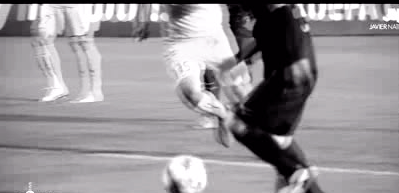
\includegraphics[scale=1]{imagenes/art1.png}

\subsection{Interpolación por Splines}

\begin{itemize}
\item Con seguridad, este hasta ahora es el método que genera los videos más fluidos.
\item Los movimientos de las cosas parecen naturales y no hay congelamientos ni transformaciones bruscas.
\item Esto se lo atribuimos a que el método en sí aprovecha todos los datos del pixel a tráves del tiempo para producir resultados mejores que tienen que ver con el marco teórico que le dan los polinomio interpoladores de Lagrange.
\item Eso si, siguen habiendo imágenes falsas a causa del movimiento y no son menores pero si ligeramente mejores que en la interpolación lineal.
\item Por ejemplo, en la instancia \textbf{skate}, los resultados son del estilo:
\end{itemize}

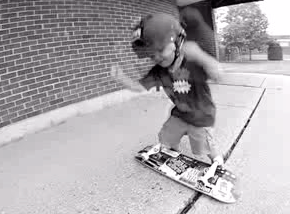
\includegraphics[scale=1]{imagenes/art2.png}

\subsection{Interpolación por Splines de a bloques de 4 pixeles}

\begin{itemize}
\item En este caso parece haber un retroceso de calidad con respecto al método anterior.
\item Los movimientos de las cosas parecen naturales.
\item Pero si hay congelamientos.
\item En particular, en el video \textbf{Messi} se nota claramente como la pelota se congela en algunos momentos.
\item Esto era de esperarse debido a los bloques de tamaño fijo ubicados a través del tiempo.
\end{itemize}
